% \section*{Appendix A. Project cost}

% \begin{table}[hb!]
% \centering
%  \renewcommand\thetable{A.1}
% \caption{Project cost}
% {
% \renewcommand{\arraystretch}{2}
% \begin{tabular}{ c|r|r }
% \hline           
%  {\textbf{Expense}} & \pbox{3cm}{\textbf{SUM (MDL)}} & \pbox{4cm}{\textbf{Percentage (\%)}} \\ \hline \hline
% {Direct expenses} & {122942} & {48.73} \\ \hline 
% {Salary expenses} & {95040} & {37.64} \\ \hline 
% {Social fund expenses} & {21859} & {8.65} \\ \hline 
% {Indirect expenses} & {5638} & {2.23} \\ \hline 
% {Medical insurance expenses} & {3801} & {1.50} \\ \hline 
% {Asset wear expenses} & {3178} & {1.25} \\ \hline 
% {\textbf{Total product cost}} & \pbox{3cm}{\textbf{252458}} & \pbox{3cm}{\textbf{100.00}} \\ \hline

% \end{tabular}
% }
% \label{project}
% \end{table}

% \newpage

\section*{Appendix A. UML Diagrams}
\phantomsection

% \subsection*{Appendix A: UML Diagrams}

      \begin{figure}[h!]
        \centering
        \subfloat[ Robot's use case]
         {
         \label{useCase1}
          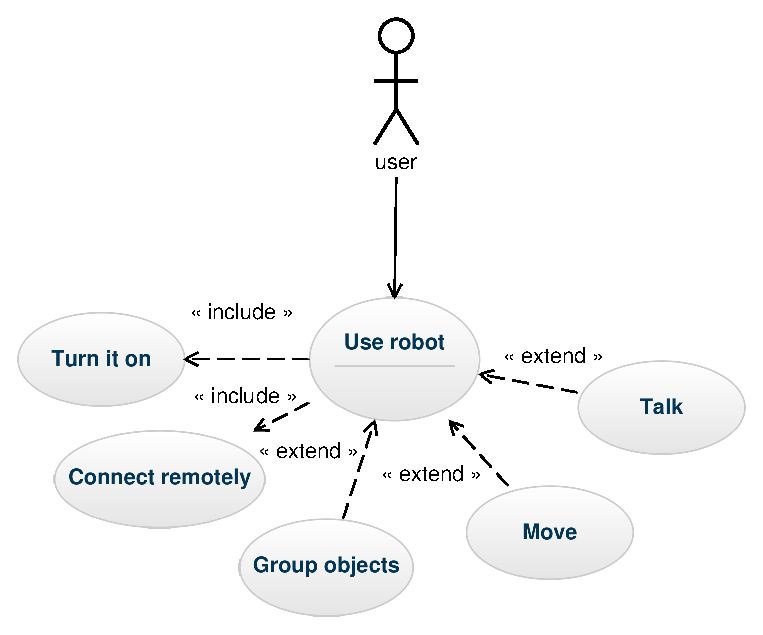
\includegraphics[width=0.45\linewidth]{useCase1.eps}
         }
        \hfil 
        \subfloat[ Group objects use case]
         {
          \label{useCase2}
          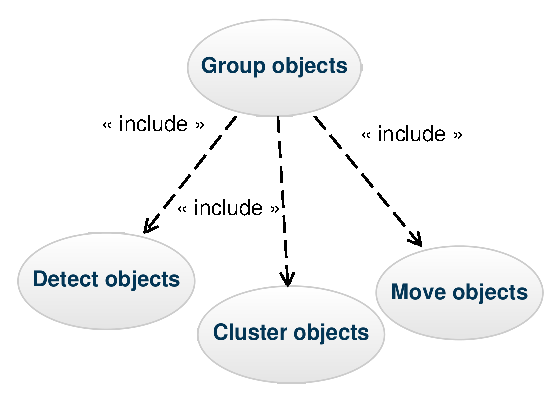
\includegraphics[width=0.45\linewidth]{useCase2.eps} 
         }
         \renewcommand\thefigure{B.1}
        \caption{ Use cases I}
        \label{useCases1}
      \end{figure}

            \begin{figure}[h!]
        \centering
        \subfloat[ Detect objects use case]
         {
         \label{useCase3}
          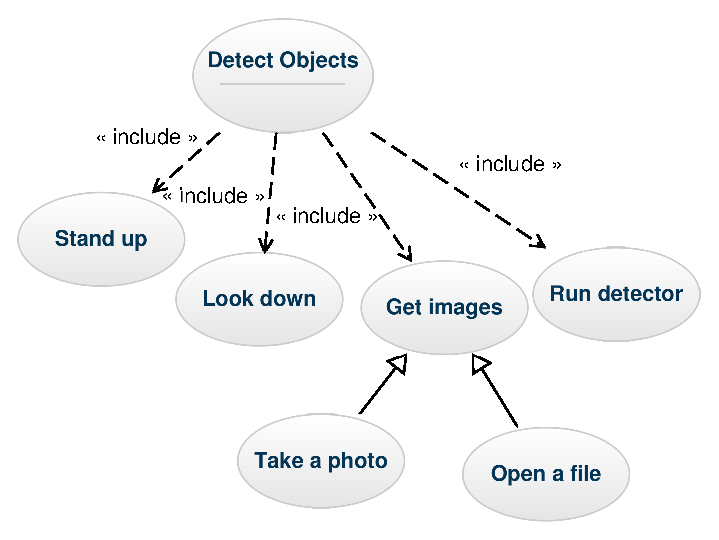
\includegraphics[width=0.45\linewidth]{useCase3.eps}
         }
        \hfil 
        \subfloat[ Move objects use case]
         {
          \label{useCase3}
          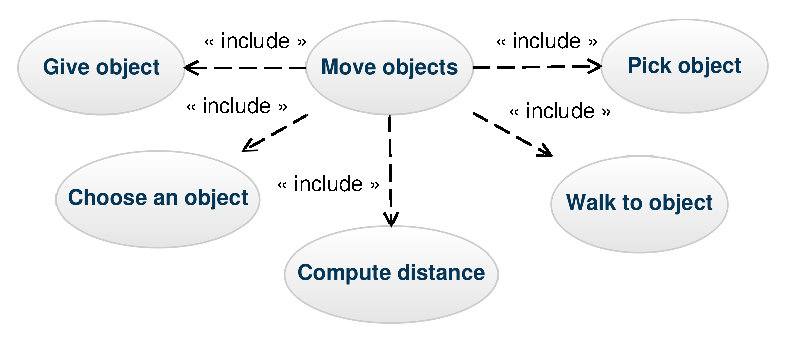
\includegraphics[width=0.45\linewidth]{useCase4.eps} 
         }
         \renewcommand\thefigure{B.2}
        \caption{ Use cases II}
        \label{useCases2}
      \end{figure}

% \begin{figure}[!ht]
% \renewcommand\thefigure{A.1}
% \centering
% 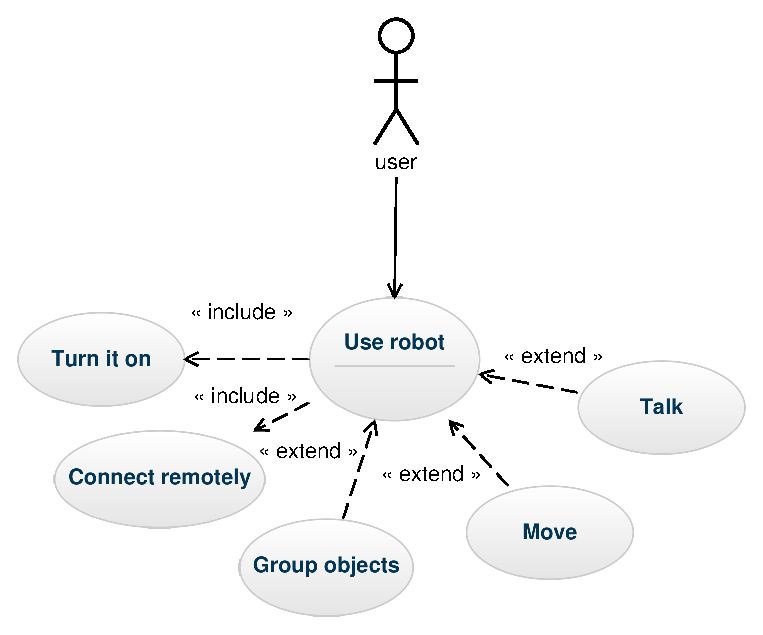
\includegraphics[scale=0.8]{useCase1.eps}
% \caption{Robot's use case}\label{useCase1}
% \end{figure}

% \begin{figure}[!hb]
% \renewcommand\thefigure{A.2}
% \centering
% 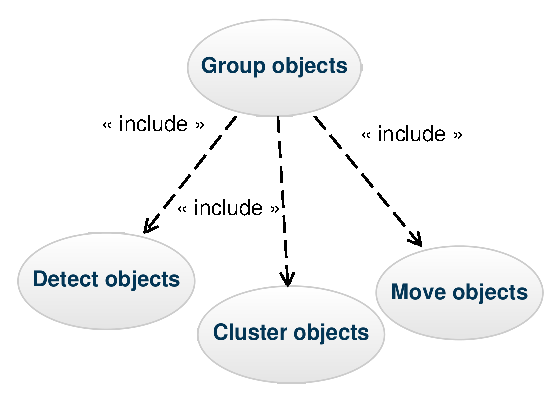
\includegraphics[scale=0.8]{useCase2.eps}
% \caption{Group objects use case}\label{useCase2}
% \end{figure}

% \begin{figure}[!ht]
% \renewcommand\thefigure{A.3}
% \centering
% 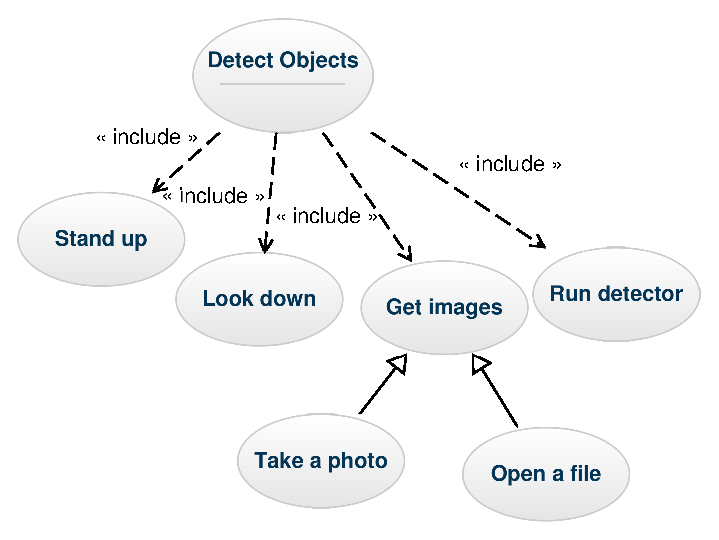
\includegraphics[scale=0.8]{useCase3.eps}
% \caption{Detect objects use case}\label{useCase3}
% \end{figure}

% \begin{figure}[!hb]
% \renewcommand\thefigure{A.4}
% \centering
% 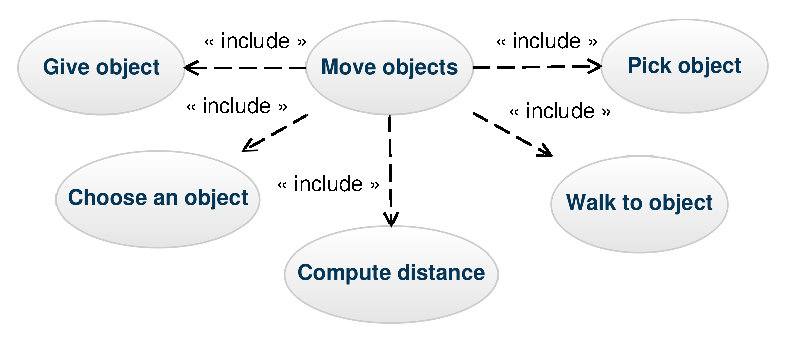
\includegraphics[scale=0.8]{useCase4.eps}
% \caption{Move objects use case}\label{useCase4}
% \end{figure}

\begin{figure}[!ht]
\renewcommand\thefigure{B.3}
\centering
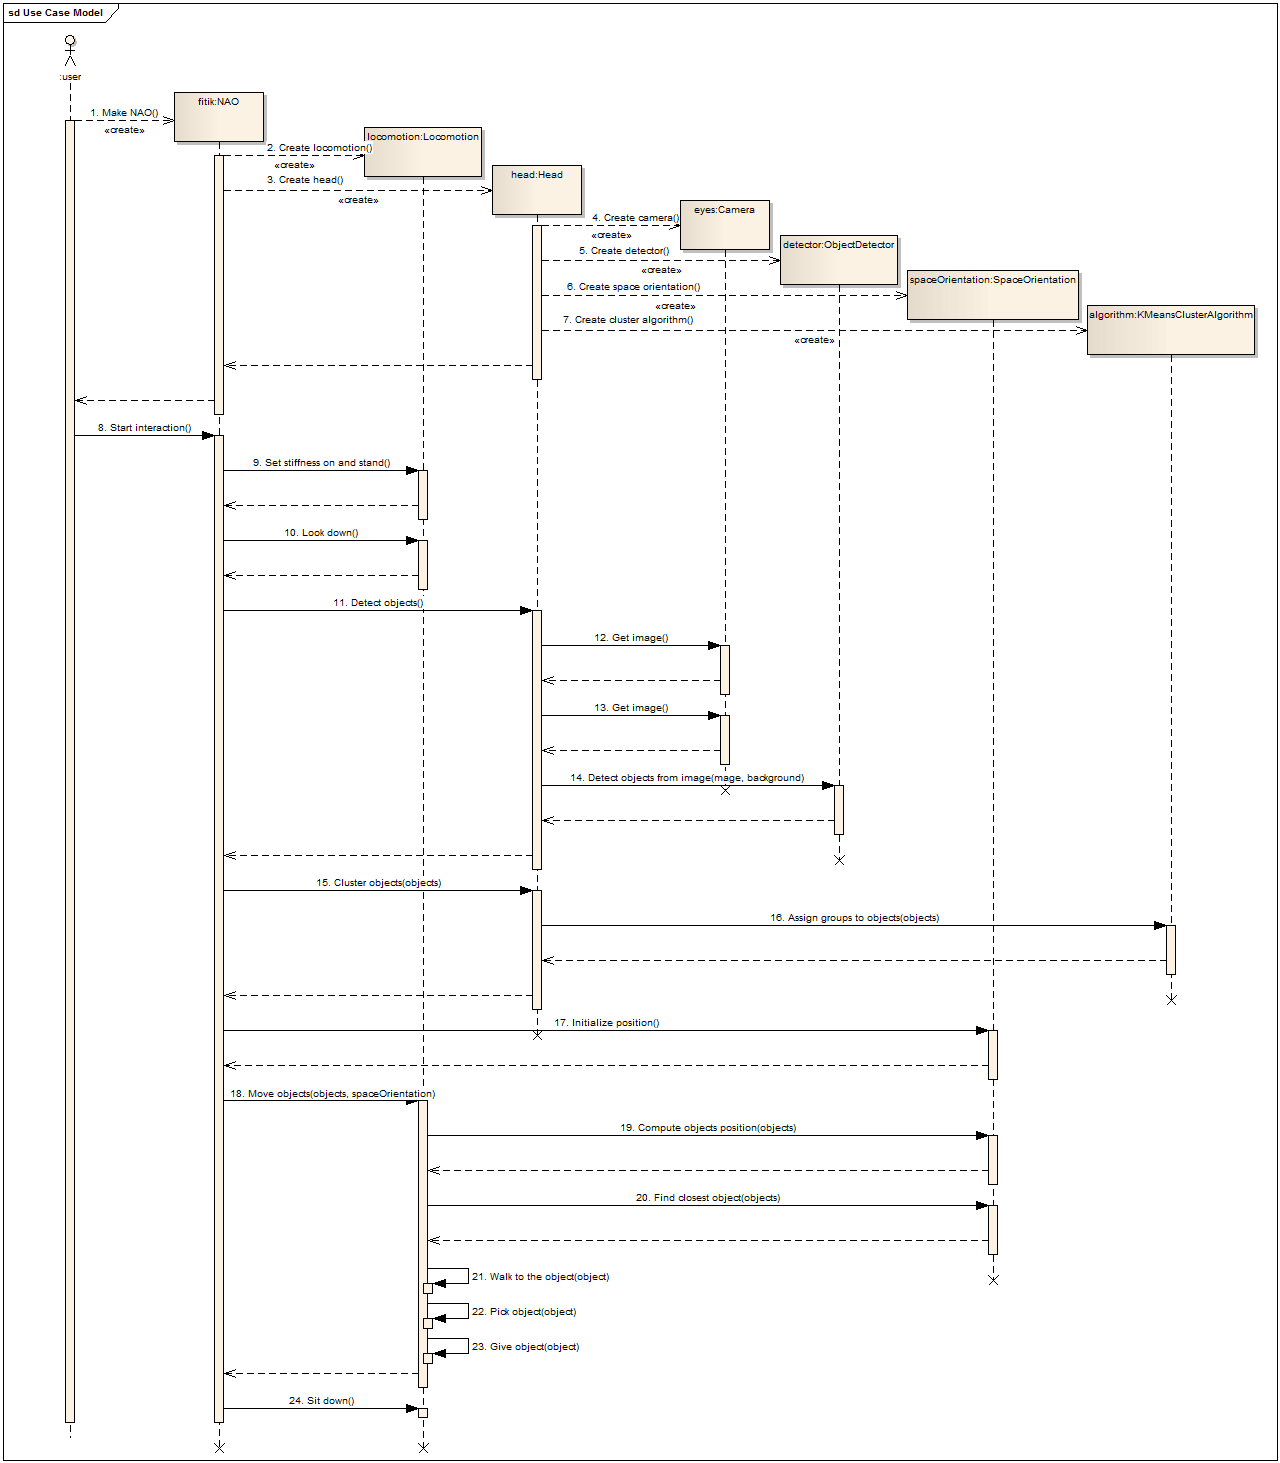
\includegraphics[width=\linewidth]{sequence.png}
\caption{A model of interaction between objects}\label{sequence}
\end{figure}

\begin{figure}[!hb]
\renewcommand\thefigure{B.4}
\centering
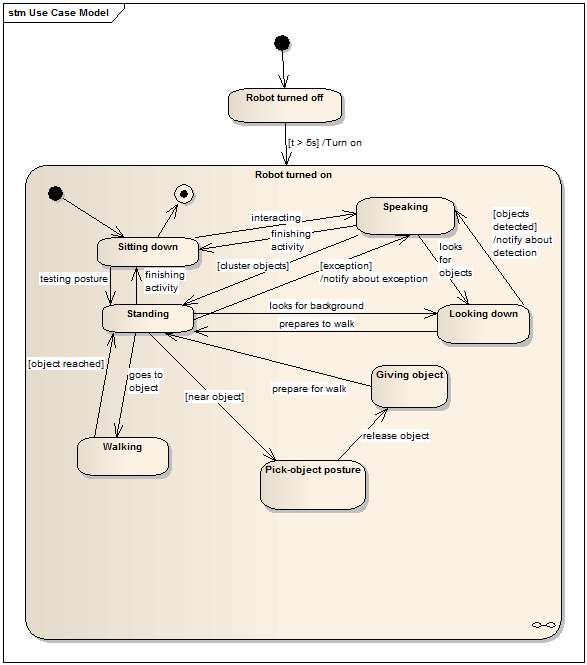
\includegraphics[scale=1]{state.png}
\caption{Robot's states}\label{state}
\end{figure}

\begin{figure}[!ht]
\renewcommand\thefigure{B.5}
\centering
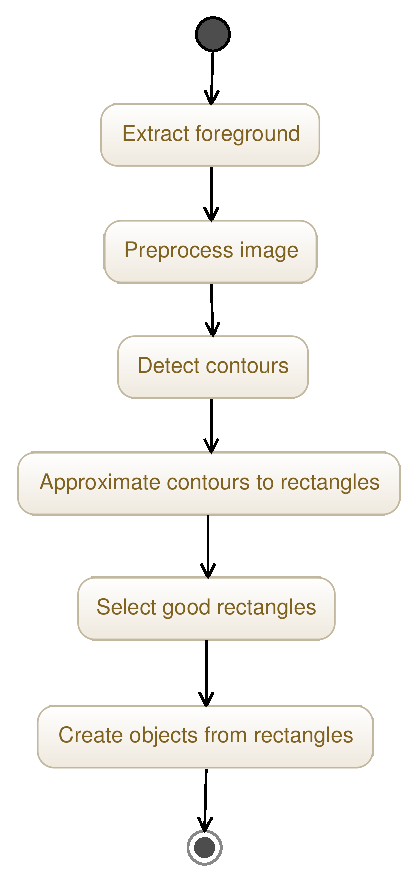
\includegraphics[scale=0.9]{activityObjectDetection.eps}
\caption{Object detection algorithm's steps}\label{activity1}
\end{figure}

\begin{figure}[!hb]
\renewcommand\thefigure{B.6}
\centering
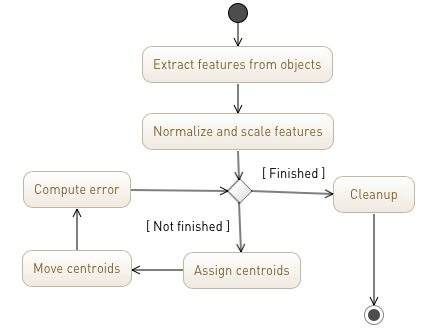
\includegraphics[scale=0.7]{activityCluster.png}
\caption{Clustering algorithm's steps}\label{activity2}
\end{figure}



\clearpage

\section*{Appendix B. Source Code}
\phantomsection
% \renewcommand\thelisting{A.1}
	\lstinputlisting[language=C++, title={SpaceOrientation class interface}, label=list21]{../SrcCode/SpaceOrientation.h}

	\lstinputlisting[language=C++, title={SpaceOrientation class implementation}, label=list22]{../SrcCode/SpaceOrientation.cpp}

	\lstinputlisting[language=C++, title={Head class interface}, label=list23]{../SrcCode/Head.h}

	\lstinputlisting[language=C++, title={Head class implementation}, label=list24]{../SrcCode/Head.cpp}

	\lstinputlisting[language=C++, title={NAO class interface}, label=list25]{../SrcCode/NAO.h}

	\lstinputlisting[language=C++, title={NAO class implementation}, label=list26]{../SrcCode/NAO.cpp}

	\lstinputlisting[language=C++, title={Main file}, label=list27]{../SrcCode/main.cpp}

% 	% \lstinputlisting[language=C++, title={Image class interface}, caption={Source code}, label=list4]{../SrcCode/Image.h}

% 	% \lstinputlisting[language=C++, title={Image class implementation}, label=list4]{../SrcCode/Image.cpp}

% 	% \lstinputlisting[language=C++, title={AbstractImageFetcher class interface}, label=list4]{../SrcCode/AbstractImageFetcher.h}

% 	% \lstinputlisting[language=C++, title={AbstractImageFetcher class implementation}, label=list4]{../SrcCode/AbstractImageFetcher.cpp}

% 	% \lstinputlisting[language=C++, title={ImageFetcherOnOSX class interface}, label=list4]{../SrcCode/ImageFetcherOnOSX.h}

% 	% \lstinputlisting[language=C++, title={ImageFetcherOnOSX class implementation}, label=list4]{../SrcCode/ImageFetcherOnOSX.cpp}

% 	% \lstinputlisting[language=C++, title={Camera class interface}, label=list4]{../SrcCode/Camera.h}

% 	% \lstinputlisting[language=C++, title={Camera class implementation}, label=list4]{../SrcCode/Camera.cpp}		

% 	% \lstinputlisting[language=C++, title={Object class interface}, label=list4]{../SrcCode/Object.h}

% 	% \lstinputlisting[language=C++, title={Object class implementation}, label=list4]{../SrcCode/Object.cpp}		

% 	% \lstinputlisting[language=C++, title={ObjectDetector class interface}, label=list4]{../SrcCode/ObjectDetector.h}

% 	% \lstinputlisting[language=C++, title={ObjectDetector class implementation}, label=list4]{../SrcCode/ObjectDetector.cpp}

% 	% \lstinputlisting[language=C++, title={AbstractClusterAlgorithm class interface}, label=list4]{../SrcCode/AbstractClusterAlgorithm.h}

% 	% \lstinputlisting[language=C++, title={AbstractClusterAlgorithm class implementation}, label=list4]{../SrcCode/AbstractClusterAlgorithm.cpp}

% 	% \lstinputlisting[language=C++, title={ObjectDetector class interface}, label=list4]{../SrcCode/ObjectDetector.h}

% 	% \lstinputlisting[language=C++, title={ObjectDetector class implementation}, label=list4]{../SrcCode/ObjectDetector.cpp}

% 	% \lstinputlisting[language=C++, title={KMeansClusteringAlgorithm class interface}, label=list4]{../SrcCode/KMeansClusteringAlgorithm.h}

% 	% \lstinputlisting[language=C++, title={KMeansClusteringAlgorithm class implementation}, label=list4]{../SrcCode/KMeansClusteringAlgorithm.cpp}

% 	% \lstinputlisting[language=C++, title={Speech class interface}, label=list4]{../SrcCode/Speech.h}

% 	% \lstinputlisting[language=C++, title={Speech class implementation}, label=list4]{../SrcCode/SpeechBig.cpp}

% 	% \lstinputlisting[language=C++, title={Head class interface}, label=list4]{../SrcCode/Head.h}

% 	% \lstinputlisting[language=C++, title={Head class implementation}, label=list4]{../SrcCode/Head.cpp}

% 	% \lstinputlisting[language=C++, title={CustomMoves class interface}, label=list4]{../SrcCode/CustomMoves.h}

% 	% \lstinputlisting[language=C++, title={CustomMoves class implementation}, label=list4]{../SrcCode/CustomMoves.cpp}

% 	% \lstinputlisting[language=C++, title={Locomotion class interface}, label=list4]{../SrcCode/Locomotion.h}

% 	% \lstinputlisting[language=C++, title={Locomotion class implementation}, label=list4]{../SrcCode/Locomotion.cpp}

% 	% \lstinputlisting[language=C++, title={SpaceOrientation class interface}, label=list4]{../SrcCode/SpaceOrientation.h}

% 	% \lstinputlisting[language=C++, title={SpaceOrientation class implementation}, label=list4]{../SrcCode/SpaceOrientation.cpp}




	






\clearpage



